\documentclass[../book.tex]{subfiles}
\graphicspath{{\subfix{../images/}}}

\begin{document}
\chapter{Further Piece-wise Functions}
\begin{introduction}[Contents]
\item Floor and Ceiling Functions
\item Problem-Solving with the Floor and Ceiling Functions
\end{introduction}
\noindent The goal of this chapter is to introduce the floor and ceiling functions, which are two rounding functions that can be helpful for problem solving.  Being able to solve problems like these will improve your ability to solve other types of piece-wise functions.
\section{Floor and Ceiling Functions}
\noindent This section covers the \textit{floor} and \textit{ceiling} functions.  These are two functions that you may have never heard of before, but they can be quite useful.  The goal of these functions is to input a decimal and return the next integer less than or greater than the function. 
\begin{definition}{The Floor and Ceiling Functions}{fnc}
Given a real constant $x$, define the floor and ceiling function as follows:\begin{itemize}
    \item The \textbf{floor} of $x$ is the greatest integer less than or equal to $x$.  This is also called the \underline{greatest integer function}.  It is denoted by $\lfloor{x}\rfloor$.
    \item The \textbf{ceiling} of $x$ is the least integer greater than or equal to $x$.  This is also called the \underline{least integer function}.  It is denoted by $\lceil{x}\rceil$.
\end{itemize}
\end{definition}
\begin{remark}
Some texts will use $[x]$ as the floor function.  We won't do this to avoid confusion.
\end{remark}
We will also define the \textit{fractional part} of $x$ as subtracting the integer component from $x$.  It is defined as $x-\lfloor{x}\rfloor$, and is denoted by $\{x\}$.

Here are some examples of the floor, ceiling, and fractional parts of $x$.\begin{align*}
    \lfloor{3}\rfloor=3 \hspace{30mm} \lceil{3}\rceil&=3 \hspace{30mm} \{3\}=0 \\
    \lfloor{6.25}\rfloor=6 \hspace{25mm} \lceil{6.25}\rceil&=7 \hspace{25mm} \{6.25\}=0.25 \\
    \lfloor{-6.25}\rfloor=-7 \hspace{19mm} \lceil{-6.25}\rceil&=-6 \hspace{19mm} \{-6.25\}=0.75 \\
    \lfloor{\pi}\rfloor=3 \hspace{30mm} \lceil{\pi}\rceil&=4 \hspace{30mm} \{\pi\}=\pi-3
\end{align*}
Let's consider the graphs of each of the functions.  For the floor function, for all real values of $x$ between $n$ and $n+1$, $\lfloor{x}\rfloor=n$.  This if we continue this for various integer values of $n$, we get a step-like graph. This follows the same logic for the ceiling function.  For the fractional part function, it follows the step-like graph; however, it has a slope.  Consider the case when $0\leq x<1$.  In this case, $y=x$, meaning that there's a slope of $1$.  This will continue for every iteration.

Below are the graphs.

\begin{figure}[!h]
    \centering
    \begin{tikzpicture}[scale=0.75,yscale=0.75]
    \tkzInit[xmin = -5, xmax = 5, ymin = -5, ymax = 5]
    \tkzAxeXY
    \foreach \a in {-5,...,5}{
        \draw[blue] (\a, \a) -- (\a + 1, \a);
        \node [circle, draw, fill=none, line width = .5pt, color = blue, inner sep = 0pt, minimum size = 3pt] (ca) at (\a, \a) {};
        \node [circle, draw, fill, line width = .5pt, color = blue, inner sep = 0pt, minimum size = 3pt] (ca) at (\a + 1, \a) {};
    }
    \end{tikzpicture} $y(x)=\lfloor{x}\rfloor$
    \begin{tikzpicture}[scale=0.75,yscale=0.75]
    \tkzInit[xmin = -5, xmax = 5, ymin = -5, ymax = 5]
    \tkzAxeXY
    \foreach \a in {-4,...,5}{
        \draw[blue] (\a - 1, \a) -- (\a, \a);
        \node [circle, draw, fill=none, line width = .5pt, color = blue, inner sep = 0pt, minimum size = 3pt] (ca) at (\a-1, \a) {};
        \node [circle, draw, fill, line width = .5pt, color = blue, inner sep = 0pt, minimum size = 3pt] (ca) at (\a, \a) {};
    }
    \end{tikzpicture} $y(x)=\lceil{x}\rceil$
    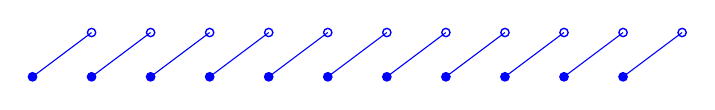
\begin{tikzpicture}[scale=0.75,yscale=0.75]
    \tkzInit[xmin = -5, xmax = 5, ymin = -5, ymax = 5]
    \tkzAxeXY
    \foreach \a in {-5,...,5}{
        \draw[blue] (\a, 0) -- (\a + 1, 1);
        \node [circle, draw, fill, line width = .5pt, color = blue, inner sep = 0pt, minimum size = 3pt] (ca) at (\a, 0) {};
        \node [circle, draw, fill=none, line width = .5pt, color = blue, inner sep = 0pt, minimum size = 3pt] (ca) at (\a + 1, 1) {};
    }
    \end{tikzpicture} $y(x)=\{x\}$
\end{figure}

Now, let's work with these functions to solve some problems.  Most of the problems for this section will focus on the floor function, since it's the most common.
\begin{example}
Compute $\lfloor{\log_2(1000)\rfloor}$.
\end{example}
\begin{solution}
Let $\lfloor{\log_2(1000)\rfloor}=n$.  This means that we can set the inequality $$n\leq\lfloor{\log_2(1000)\rfloor}<n+1,$$ where $n\in\mathbb{Z}$.  Converting the inequality to exponential, we get $$2^n\leq 1000<2^{n+1}.$$  Since $512=2^9\leq 1000<2^{10}=1024$, this means that $n=\lfloor{\log_2(1000)\rfloor}=9$. $\Box$
\end{solution}
\begin{example}
Find all $x$ such that $\left\lfloor{3x+\dfrac{1}{2}}\right\rfloor=7$.
\end{example}
\begin{solution}
Because $\left\lfloor{3x+\dfrac{1}{2}}\right\rfloor=7$, we know that $3x+\dfrac{1}{2}$ is between $7$ and $8$, meaning $$7\leq 3x+\dfrac{1}{2}<8.$$  This is something we know how to solve.  Solving this gives us $$7\leq 3x+\dfrac{1}{2}<8 \implies \dfrac{13}{2}\leq x<\dfrac{15}{2} \implies \dfrac{13}{6}\leq x<\dfrac{5}{2}.$$ $\Box$
\end{solution}
\begin{example}
Find all $x$ such that $2<\lfloor{4x-5}\rfloor\leq 8$.
\end{example}
\begin{solution}
Since $\lfloor{4x-5}\rfloor$ must be an integer, we can change the lower bound to the next integer, $4$.  This makes the inequality $4\leq \lfloor{4x-5}\rfloor\leq 8$.  This means that $4x-5$ is a number between $4$ and $9$, so we can remove the floor notation and write $4\leq 4x-5<9$.  Solving for $x$ gives $$4\leq 4x-5<9 \implies 9\leq 4x<14 \implies \dfrac{9}{4}\leq x<\dfrac{7}{2}.$$ $\Box$
\end{solution}
The final type of problem that the floor function is used for is evaluating the approximate value of large operations without a calculator.  We will try one example of this.
\begin{example}
Evaluate $\left\lfloor{\dfrac{2007^3}{2005 \cdot 2006}-\dfrac{2005^3}{2006\cdot 2007}}\right\rfloor$ without a calculator.
\end{example}
\begin{solution}
We will not multiply this all out; it would take way too long and there's too many places to make mistakes.  Instead, we will use some algebra to simplify it.  If we let $n=2005$, we can write the expression in terms of $n$ and then simplify from there.  \begin{align*}
    \dfrac{2007^3}{2005 \cdot 2006}-\dfrac{2005^3}{2006\cdot 2007}&=\dfrac{(n+2)^3}{n(n+1)}-\dfrac{n^3}{(n+1)(n+2)}=\dfrac{(n+2)^4-n^4}{n(n+1)(n+2)} \\
    &=\dfrac{8n^3+24n^2+32n+16}{n(n+1)(n+2)}=\dfrac{8(n+1)(n^2+2n+2)}{n(n+1)(n+2)} \\
    &=\dfrac{8(n^2+2n+2)}{n(n+2)}=\dfrac{8n(n+2)+16}{n(n+2)} \\
    &=8+\dfrac{16}{n(n+2)} 
\end{align*}
We've made significant process!  Now, what to do with the $\dfrac{16}{n(n+2)}$ term? Well, at $n=2005$, we know that $0<\dfrac{16}{n(n+2)}<1$, meaning that $$\left\lfloor{\dfrac{2007^3}{2005 \cdot 2006}-\dfrac{2005^3}{2006\cdot 2007}}\right\rfloor=8.$$ $\Box$
\end{solution}
Those are the basic problems that you'll experience when it comes to the floor function.  Now, let's look at some harder problems using the same methods.
\section{Problem-Solving with the Floor Function}
\noindent The goal of this section is to over various approaches when it comes to the floor function.  These aren't new techniques, but rather are different ways of looking at harder problems using the same techniques.
\begin{example}
Find all values of $x$ such that $x+\lfloor{x}\rfloor=6.7$.
\end{example}
\begin{solution}
The easiest way to do this is to split the answer into two parts (the integer and the fractional part). We know that the only way to get the $0.7$ part of the answer is from the $x$, meaning $x$ must have $0.7$ in it.  That leaves the integer component of $x$ and $\lfloor{x}\rfloor$.  Since both must be the same, we know that $\lfloor{x}\rfloor=3$.  This means that $x=3.7$.

If you don't understand how that works, note that $x=\lfloor{x}\rfloor+\{x\}$.  This way, we get $2\lfloor{x}\rfloor+\{x\}=6.7$, which makes $x=3.7$ by splitting the equation. $\Box$
\end{solution}
\begin{example}
Find all real numbers $x$ such that $\lfloor{x}\rfloor=5x-14$.
\end{example}
\begin{solution}
Again, for this one, we will use the idea that $x=\lfloor{x}\rfloor+\{x\}$.  This gives us $$\lfloor{x}\rfloor=5\lfloor{x}\rfloor+5\{x\}-14.$$  Solving for $\{x\}$, we get $$\{x\}=\dfrac{14-4\lfloor{x}\rfloor}{5}.$$  Since $0\leq \{x\}<1$, we have $0\leq \dfrac{14-4\lfloor{x}\rfloor}{5}<1$.  Solving this for $x$ gives us $$0\leq 14-4\lfloor{x}\rfloor<5 \implies \dfrac{9}{4}<\lfloor{x}\rfloor\leq \dfrac{7}{2}.$$  The only integer on the interval is $3$, meaning that $\lfloor{x}\rfloor=3$.  Therefore, $\{x\}=\dfrac{14-4\cdot 3}{5}=\dfrac{2}{5}$.  Thus, $x=\lfloor{x}\rfloor+\{x\}=\dfrac{17}{5}=3.4$. $\Box$
\end{solution}
For the final problem in this chapter, we are going to do a summation.  Don't be alarmed; this is not a difficult problem.  We just need to understand what we are adding and find a way to evaluate an equivalent sum that's easier to add.
\begin{example}
Find $\displaystyle \sum_{k=1}^{99}{\left\lfloor{\sqrt{k}}\right\rfloor}$.
\end{example}
\begin{solution}
Let's expand the summation to take a look at what we are adding: $$\sum_{k=1}^{99}{\left\lfloor{\sqrt{k}}\right\rfloor}=\left\lfloor{\sqrt{1}}\right\rfloor+\left\lfloor{\sqrt{2}}\right\rfloor+\left\lfloor{\sqrt{3}}\right\rfloor+\left\lfloor{\sqrt{4}}\right\rfloor+\left\lfloor{\sqrt{5}}\right\rfloor+\cdots+\left\lfloor{\sqrt{99}}\right\rfloor.$$
The first way to do this is brute force.  We know that $\left\lfloor{\sqrt{1}}\right\rfloor=1$, $\left\lfloor{\sqrt{2}}\right\rfloor=\left\lfloor{\sqrt{3}}\right\rfloor=1$.  The next term is then $\left\lfloor{\sqrt{4}}\right\rfloor=\left\lfloor{\sqrt{5}}\right\rfloor=\left\lfloor{\sqrt{6}}\right\rfloor=\left\lfloor{\sqrt{7}}\right\rfloor=\left\lfloor{\sqrt{8}}\right\rfloor=2$, and then $\left\lfloor{\sqrt{9}}\right\rfloor=3$.

There is a clear pattern here.  We first notice that we can solve this by counting the number of values between the perfect squares and then multiply by their floor function (since they're all the same).  This is the simple way to do it.  We are going to follow this method but provide a more mathematical explanation.

Our goal is to find all integers $k$ such that $\left\lfloor{\sqrt{k}}\right\rfloor=m$, where $m$ is a positive integer.  This means that $m\leq \sqrt{k}<m+1$, so $m^2\leq k<(m+1)^2$.  Counting the number of integers in this list, $k$ must be one of $m^2$, $m^2+1$, $m^2+2$, $\ldots$, $(m+1)^2-1$.  There are $((m+1)^2-1)-(m^2)+1=2m+1$ integers in this list.  These integers are then multiplied by $m$.  There are $9$ perfect squares in the range, meaning $m$ ranges from $1$ to $9$.

This means that we can rewrite the given summation as $$S=\sum_{k=1}^{99}{\left\lfloor{\sqrt{k}}\right\rfloor}=\sum_{m=1}^{9}{m(2m+1)}.$$  Evaluating the sum by plugging in each value of $m$, we get $$S=3+10+21+36+55+78+105+136+171=615.$$ $\Box$
\end{solution}
This is all we have to cover.  This chapter was somewhat on the short side; we reviewed one function and introduced another.  Although you won't see the floor function as often in regular mathematics classes, it's a good skill to know how to use and implement.  Courses that focus on competition preparation will go into much greater detail on these functions.
\begin{reviewset}
\item Simplify $\left|x-\sqrt{(x-9)^2}\right|$ for all $x<0$. \vspace{3mm}
\item Show that $\lceil{x}\rceil=-\lfloor{-x}\rfloor$ for all $x\in\mathbb{R}$. \vspace{3mm}
\item Find $f^{-1}(x)$ if $f(x)=x|x|+2$. \vspace{3mm}
\item Find all constants $c$ such that $|cx-1|+|x^2-x-2|=0$ has a solution in $x$. \vspace{3mm}
\item Let $a$ and $b$ be distinct real numbers.  Find $x$ in terms of $a$ and $b$ such that $|x-a|=|x-b|$. \vspace{3mm}
\item Find all ordered pairs $(x.y)$ such that $|x|+|y|=10$ and $xy=24$. \vspace{3mm}
\item Let $a$, $b$, and $c$ be real numbers such that $|a|=|b-2|$, $|b|=|c-2|$ and $|c|=|a-2|$.  Prove that $a+b+c=3$.  \vspace{3mm}
\item Determine whether the following functions are continuous. Then, determine if the function has an inverse; if so, find it. \newline
(a) $f(x)=\begin{cases} 4x & x<5 \\ 5/x & x\geq 5 \end{cases}$. \hspace{30mm}
(b) $g(x)=\begin{cases} 2x & x<2 \\ 2^x & x\geq 2 \end{cases}$. \vspace{3mm}
\item Evaluate $\left\lfloor{\log_2\sqrt{999}}\right\rfloor$ without the use of a calculator.  \vspace{3mm}
\item How many ordered triples of integers $(a,b,c)$ satisfy $|a+b|+c=19$ and $ab+|c|=97$? \vspace{3mm}
\item Find the values of $x$ that satisfy $\left\lfloor{\sqrt{2x-7}}\right\rfloor=9$. \vspace{3mm}
\item Find all integers $x$ such that $\lfloor{x/6}\rfloor=5$. \vspace{3mm}
\item Compute $\left\lfloor{\sqrt{n^2-10n+29}}\right\rfloor$ when $n=20252025$. \vspace{3mm}
\item Find all values of $x$ such that $7x+\lfloor{2x}\rfloor=52$. \vspace{3mm}
\end{reviewset}
\begin{challengeset}
\item Find all real values of $x$ such that $\left\lfloor{\left|-x^2+10x-16\right|}\right\rfloor=1$. \vspace{3mm}
\item Find $\dfrac{\{\sqrt{3}\}^2-2\{\sqrt{2}\}^2}{\{\sqrt{3}\}-2\{\sqrt{2}\}}$ without a calculator. \vspace{3mm}
\item Graph $f(x)=\lfloor{x}\rfloor+\lceil{x}\rceil$ and $g(x)=\lceil{x}\rceil-\lfloor{x}\rfloor$. \vspace{3mm}
\item Find the largest real positive number $\delta$ such that $\left|\sqrt{x}-2\right|<0.1$ if $|x-4|<\delta$. \vspace{3mm}
\item Let $S_n=\lfloor{1}\rfloor+\lfloor{2}\rfloor+\lfloor{3}\rfloor+\cdots+\lfloor{n}\rfloor$ where $n\in\mathbb{Z}$.  Find the largest value of $k<2021$ such that $S_{2021}-S_k$ is a perfect square. \vspace{3mm}
\item What positive, real number $x$ has the property that $x$, $\lfloor{x}\rfloor$, and $x-\lfloor{x}\rfloor$ form a geometric progression?\vspace{3mm}
\item Find the domain of $f(x)=\dfrac{\sqrt{64-x^2}}{\sqrt[4]{16-|2x+5|}}$. \vspace{3mm}
\item Find the smallest real number $x$ such that $\dfrac{x}{\lfloor{x}\rfloor}=\dfrac{2002}{2003}$. \vspace{3mm}
\item Graph $f(x)=\lfloor{2x}\rfloor+\lfloor{4x}\rfloor+\lfloor{6x}\rfloor+\lfloor{8x}\rfloor$. \vspace{3mm}
\item The function $f$ is defined on $\mathbb{Z}$ and satisfies $$f(n)=\begin{cases} n-3 & n\geq 1000 \\ f(f(n+5)) & n<1000\end{cases}.$$  Find $f(84)$. \vspace{3mm}
\item Define $f(n)$ by $$\begin{cases} n/2 & \text{if } n \text{ is even} \\ (n+1023)/2 & \text{ if } n \text{ is odd} \end{cases}.$$  Find the least positive integer such that $f(f(f(f(f(n)))))=n$. (HINT: Experiment with small values of $n$.  Also, use the fact that there are lots of $2$'s.  How could we go about writing $n$ to make this problem easier?) \vspace{3mm}
\end{challengeset}
\end{document}